%!TEX root = ../main.tex

\section{Introduction}

\begin{enumerate}
    \item \textbf{Financial Instrument:} A legal contract having monetary value. It's usually an asset on one entity and liability to other. Example: Check, Gold future contract, shares, bonds, personal loans, etc.
     Every financial security and product is a financial insturment but not the other way around.
    \item \textbf{Financial Security:} A specific kind of financial instrument that is fungible and negotiable. 
    Fungible means it can be swapped for another of the same kind, and negotiable means that it can be readily traded on private of public markets.
    Examples: Bonds, and Stocks.
    \item \textbf{Financial Product:} Package or service created by a financial institution to help individuals save, invest, or protect their money.
    Examples: Life insurance policy, mutual funds, etc.
    \item \textbf{Stock:} General term used to describe the ownership certificate of any firm.
    \item \textbf{Share:} Smallest unit of a company's stock. Stock of the substance, and share is the unit. 
    \item \textbf{Systemic Risk:} Risk that a default by one financial institution will create a "ripple effect" that leads to defaults by other financial institutions and threaten the stability of the financial system.
    \item \textbf{Forward Contract:} An agreeement to buy or sell an asset at a certain future time for a certain price.
    Payoff from a long position in a forward contract is $S_T - K$.
    \item \textbf{Futures Contracts:} Forward contract, but is standardized and traded on an exchange.
    \item \textbf{Options:} There are two types of options:
    \begin{enumerate}
        \item \textbf{Call Option:} Gives the holder the right to buy the underlying asset by a certain date for a certain price.
        \item \textbf{Put Option:} Gives the holder the right to sell the underlying asset by a certain date for a certain price.
    \end{enumerate}
    \item American options can be exercised at any time up to the expiration date.
    \item American and European here do not refer to the location of the option or the exchange.
    \item Buyers are referred to as having \textit{long positions}; sellers are referred to as having \textit{short positions}. 
    \item Selling an option is also known as \textit{writing the option}.
    \item \textbf{Payoffs:}
    \begin{enumerate}
        \item \textbf{Long CE:} $(S_T - K)^+$
        \item \textbf{Short CE:} $-(S_T - K)^+$
        \item \textbf{Long PE:} $(K - S_T)^+$
        \item \textbf{Short PE:} $-(K - S_T)^+$
    \end{enumerate}

    % \begin{figure}[h]
    % \centering
    % \begin{tikzpicture}[scale=0.8]
    %     % Define some common styles
    %     \tikzset{
    %         axis/.style={->,>=stealth,thick},
    %         payoff/.style={ultra thick, blue},
    %         labels/.style={font=\small}
    %     }

    %     % --- LONG CALL (Top Left) ---
    %     \begin{scope}[shift={(0,0)}]
    %         \draw[axis] (-0.5,0) -- (4,0) node[right] {$S_T$};
    %         \draw[axis] (0,-0.5) -- (0,3) node[above] {Long Call};
    %         \draw[payoff] (0,0) -- (1.5,0) -- (3.5,2);
    %         \draw[dashed] (1.5,0) node[below] {$K$} -- (1.5,0.2);
    %     \end{scope}

    %     % --- LONG PUT (Top Right) ---
    %     \begin{scope}[shift={(6,0)}]
    %         \draw[axis] (-0.5,0) -- (4,0) node[right] {$S_T$};
    %         \draw[axis] (0,-0.5) -- (0,3) node[above] {Long Put};
    %         \draw[payoff] (0,2.5) -- (2.5,0) -- (4,0);
    %         \draw[dashed] (2.5,0) node[below] {$K$} -- (2.5,0.2);
    %     \end{scope}

    %     % --- SHORT CALL (Bottom Left) ---
    %     \begin{scope}[shift={(0,-5)}]
    %         \draw[axis] (-0.5,0) -- (4,0) node[right] {$S_T$};
    %         \draw[axis] (0,-3) -- (0,1) node[above] {Short Call};
    %         \draw[payoff] (0,0) -- (1.5,0) -- (3.5,-2);
    %         \draw[dashed] (1.5,0) node[above] {$K$} -- (1.5,-0.2);
    %     \end{scope}

    %     % --- SHORT PUT (Bottom Right) ---
    %     \begin{scope}[shift={(6,-5)}]
    %         \draw[axis] (-0.5,0) -- (4,0) node[right] {$S_T$};
    %         \draw[axis] (0,-3) -- (0,1) node[above] {Short Put};
    %         \draw[payoff] (0,-2.5) -- (2.5,0) -- (4,0);
    %         \draw[dashed] (2.5,0) node[above] {$K$} -- (2.5,-0.2);
    %     \end{scope}
    % \end{tikzpicture}
    % \caption{Payoff diagrams for the four basic option positions.}
    % \end{figure}


    \item \textbf{Arbitrage:} Riskless profit.
    \item \textbf{Trading Volume:} Number of contracts traded in a day.
    \item \textbf{Open Interest:} Number of contracts outstanding.
    \item \textbf{Patterns of Future:}
    \begin{enumerate}
        \item \textbf{Normal Market:} Futures market where futures prices increase with maturity.
        \item \textbf{Inverted Market:} Futures market where futures prices decrease with maturity.
    \end{enumerate}
    \item \textbf{Orders:}
    \begin{enumerate}
        \item \textbf{Market Order:} Request that a trade be carried out immediately at the best price available in the market.
        \item \textbf{Limit Order:} Specifies a particular price. Order can be executed only at this price or at one more favourable to the trader.
        \item \textbf{Stop Order/Stop-loss Order:} Also specifies a particular price. Order is executed at the best price once a bid or ask is made at that particular price or a less favourable price.
        \item \textbf{Stop-limit order:} Combination of a stop order and a limit order. Two prices must be specified: stop price, and limit price.
        \item \textbf{Market-if-touched order/MIT:} Executed at the best available price after a trade occurs at a specified price or at a price more favourable than the specified price.
        An MIT becomes a market order once the specified price has been hit.
    \end{enumerate}
    \item \textbf{CAPM:} Expected return on asset = $R_F + \beta (R_M - R_F)$
    \item \textbf{Risk-Neutral World:} A world where investors are risk-neutral, i.e., they don't demand increased expected return to compensate for increased risk. This is in contrast with the real world, where people are risk-averse.
    Risk-neutral world has two features:
    \begin{enumerate}
        \item Expected rate of return on any investment is the risk-free rate.
        \item The discounted rate used for an expected payoff on an instrument is the risk free rate.
    \end{enumerate} 
\end{enumerate}

\begin{figure}[h]
    \centering
    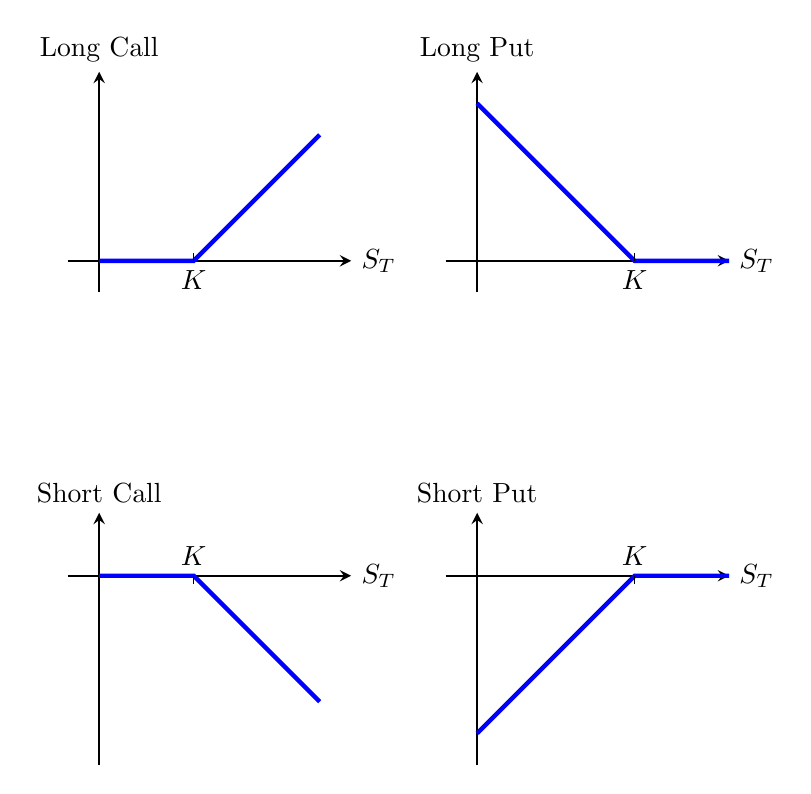
\begin{tikzpicture}[scale=0.8]
        % Define some common styles
        \tikzset{
            axis/.style={->,>=stealth,thick},
            payoff/.style={ultra thick, blue},
            labels/.style={font=\small}
        }

        % --- LONG CALL (Top Left) ---
        \begin{scope}[shift={(0,0)}]
            \draw[axis] (-0.5,0) -- (4,0) node[right] {$S_T$};
            \draw[axis] (0,-0.5) -- (0,3) node[above] {Long Call};
            \draw[payoff] (0,0) -- (1.5,0) -- (3.5,2);
            \draw[dashed] (1.5,0) node[below] {$K$} -- (1.5,0.2);
        \end{scope}

        % --- LONG PUT (Top Right) ---
        \begin{scope}[shift={(6,0)}]
            \draw[axis] (-0.5,0) -- (4,0) node[right] {$S_T$};
            \draw[axis] (0,-0.5) -- (0,3) node[above] {Long Put};
            \draw[payoff] (0,2.5) -- (2.5,0) -- (4,0);
            \draw[dashed] (2.5,0) node[below] {$K$} -- (2.5,0.2);
        \end{scope}

        % --- SHORT CALL (Bottom Left) ---
        \begin{scope}[shift={(0,-5)}]
            \draw[axis] (-0.5,0) -- (4,0) node[right] {$S_T$};
            \draw[axis] (0,-3) -- (0,1) node[above] {Short Call};
            \draw[payoff] (0,0) -- (1.5,0) -- (3.5,-2);
            \draw[dashed] (1.5,0) node[above] {$K$} -- (1.5,-0.2);
        \end{scope}

        % --- SHORT PUT (Bottom Right) ---
        \begin{scope}[shift={(6,-5)}]
            \draw[axis] (-0.5,0) -- (4,0) node[right] {$S_T$};
            \draw[axis] (0,-3) -- (0,1) node[above] {Short Put};
            \draw[payoff] (0,-2.5) -- (2.5,0) -- (4,0);
            \draw[dashed] (2.5,0) node[above] {$K$} -- (2.5,-0.2);
        \end{scope}
    \end{tikzpicture}
    \caption{Payoff diagrams for the four basic option positions.}
\end{figure}






